\documentclass[a4paper, english, 12pt]{article}

% General packages
\usepackage{parskip}      % Vertical space on new paragraph instead of indent
\usepackage{hyperref}   % For including links
\usepackage{url}          % Allows adding url's
\usepackage[top=4cm, bottom=4cm]{geometry}     % Easier management of page dimensions
\usepackage{chngcntr}     % Customizable counters
\usepackage{enumitem}     % Can use [noitemsep] on lists to reduce spacing
\usepackage{fancyhdr}
\pagestyle{fancy}
\usepackage{afterpage} 	% Various tweaks for page breaks and stuff

% BEGIN Floats
\usepackage[bf, hang, small]{caption}	% Nicer captions for floats.
\usepackage{float}        % Allows advanced placement options for floats
% \usepackage{subfig}		% Sub-figures. Crashes with captions package
% END Floats


% BEGIN Tables
\usepackage{booktabs}		% More professional looking tables
\usepackage{tabularx}		% Allows width adjustment etc. for tables
\usepackage{multirow}		% Allows table cells to span rows or columns




% Font specific packages
\usepackage{fontspec}
\usepackage{textcomp}
\usepackage{titlesec}
\usepackage{titling}
\usepackage{inconsolata}
\usepackage[default]{droidserif}

% Specifying fonts
\setsansfont{Open Sans}
\setmainfont[Scale=0.80]{Droid Serif}
\fontspec{Inconsolata}
\setmonofont[Scale=0.80]{Inconsolata}
\newfontfamily\headingfont[]{Open Sans}
\newfontfamily\headingfont[]{Open Sans}
\titleformat*{\section}{\Large\headingfont}
\titleformat*{\subsection}{\large\headingfont}
\titleformat*{\subsubsection}{\normalsize\headingfont}
\renewcommand{\maketitlehooka}{\headingfont}



\usepackage{moreverb}     % Allows use of tables in verbatim
\usepackage{fancyvrb}     % Fancy verbatim stuff
\usepackage{listings}     % Source code listings
\usepackage[usenames,dvipsnames]{color}		% Used for colors by various other packages

% Configuring listings
\definecolor{light-gray}{RGB}{250,250,250} 	% Background color for listings
\definecolor{gray}{RGB}{100,100,100} 	% Color for line-numbers
\lstset{
	language={C},			% the language of the code
	aboveskip=1em,
	belowskip=0em,
	basicstyle=\ttfamily\footnotesize,
	backgroundcolor=\color{light-gray},
	frame=single,				% adds a frame around the code
	rulecolor=\color{black},	% frame color
	captionpos=t,				% sets the caption-position to bottom
	breaklines=true,			% sets automatic line breaking
	breakatwhitespace=false,	% automatic breaks only at whitespace?
	keepspaces=true,			% keeps spaces in text, useful for keeping indentation of code (possibly needs columns=flexible)
	tabsize=4,					% sets default tabsize to 2 spaces
	commentstyle=\color{green},	% comment style
	keywordstyle=\color{blue},	% keyword style
	stringstyle=\color{red},	% string literal style
	numbers=left,				% line-number position: none, left or right
	numbersep=5pt,				% how far the line-numbers are from the code
	numberstyle=\tiny\color{gray}, % the style that used for line-numbers
	stepnumber=2,				% step between two line-numbers.
	showspaces=false,			% show spaces everywhere with underscores
	showtabs=false,				% show tabs within strings with underscores
	showstringspaces=false,		% underline spaces within strings only
	escapeinside={\%*}{*)},		% if you want to add LaTeX within your code
	title=\lstname				% show the filename of files included with \lstinputlisting; also try caption instead of title
}

\usepackage{cite}



\title{3D Visualization of petroleum data\\ 
\vspace{6pt}\large Project 1: Visualization using OpenGL and C \\ 
 }
\author{Einar Baumann}   
\date{\today}


\begin{document}

\maketitle
\thispagestyle{empty}
\pagebreak


\section{Filereader}
\label{sec:filereader}
The file reading function was implemented in a separate header file. The method takes as input the path of the file to be read; a pointer to the matrix to store the data in; and the number of traces and samples contained in the file. The implementation is shown in Listing~\ref{lst:filereader}.

\begin{lstlisting}[label=lst:filereader, caption=SEGYReader.c]
void ReadSEGYTraceSamples (char *fileName, char *matrix, size_t traces, size_t samples)
{
  FILE* fileP = fopen(fileName, "rb");
  fseek(fileP, 3600, SEEK_SET);				// Skipping 3600 byte file header.
  for (int i = 0; i < traces; i++)
  {
    fseek(fileP, 240, SEEK_CUR);			// Skipping 240 byte trace header.
    for (int j = 0; j < samples; j++)
    {
      fread(&matrix[i*samples+j], 1, 1, fileP);
    }
  }
  fclose(fileP);
}
\end{lstlisting}

% section filereader (end)


\section{Color mapping}
\label{sec:color_mapping}
A linear color mapping from red to blue via white was used. It's illustrated in Figure~\ref{fig:scale}. To determine the color of each point the program calculates a factor determining how much each value deviates from the extremum (i.e. 128). This is then used to make the color more red or blue, depending on whether the value is negative or positive. The central parts of the implementation is shown in Listing~\ref{lst:color_map}.



\begin{lstlisting}[label=lst:color_map, caption={Part of the color mapping implementation. The shown code calculates the factor used to determine the intensity of the color, as well as RGB color mapping of positive values.} ]
element = seismic[i][j];
factor = (float) abs(element)/128.0;
if( element > 0)          // Setting positive elements to blue
{
  textureRGBArray[textureNr][3*pixelCounter]   = 255 - 255*factor;
  textureRGBArray[textureNr][3*pixelCounter+1] = 255 - 255*factor;
  textureRGBArray[textureNr][3*pixelCounter+2] = 255;
}
\end{lstlisting}

\begin{figure}[htp]
\centering
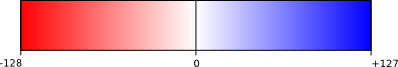
\includegraphics{graphics/scale.png}
\caption{The scale used for the color mapping.}
\label{fig:scale}
\end{figure}


% section color_mapping (end)


\section{Mipmapping and filtering}
\label{sec:mipmap_and_filter}
Screencaps of the program with mipmapping turned on and off and with different filters and zoom levels are shown in figures \ref{fig:no_mip_lin}-\ref{fig:mip_lin_zoomed-in}. 

Figures \ref{fig:no_mip_lin}, \ref{fig:mip_lin} and \ref{fig:mip_trilin} all show the same area of seismic data, but Figure \ref{fig:no_mip_lin} does not use mipmapping while \ref{fig:mip_lin} and \ref{fig:mip_trilin} do; and \ref{fig:mip_lin} and \ref{fig:mip_trilin} use different filters (linear and trilinear, respectively). We can see that the use of mipmapping and linear filtering in Figure~\ref{fig:mip_lin} results in a much smoother picture, where the lines can be more clearly seen than in the case with no mipmapping. The use of trilinear filtering in Figure~\ref{fig:mip_trilin} smooths the picture too much, making many of the lines hard to see. 

When zoomed all the way in (Figures \ref{fig:no_mip_lin_zoomed-in} and \ref{fig:mip_lin_zoomed-in}), there is no difference between the picures with and without mipmapping. This is exactly as expected because mipmapping is used when the textures contains more points than what can be fitted on the screen (i.e. when zoomed out).


\begin{figure}[htp]
\centering
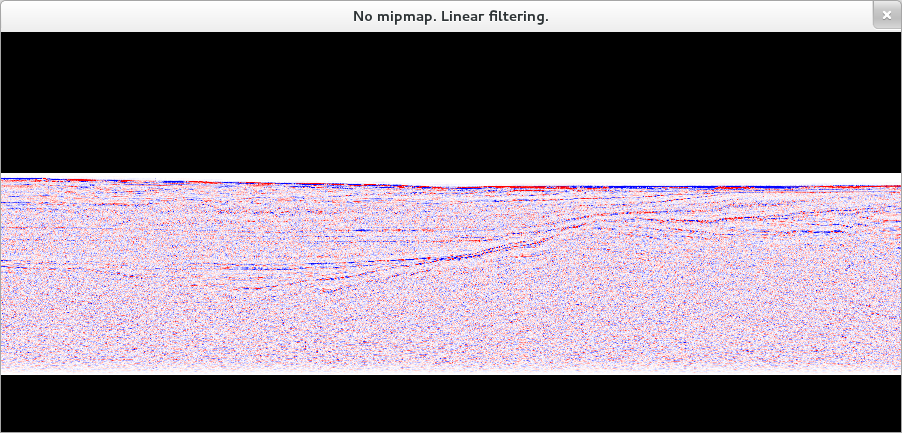
\includegraphics[clip=true, trim=10cm 5cm 10cm 6.5cm]{graphics/mip-off_linear_z0.7_x0.0_y0.0.png}
\caption{No mipmapping; linear filtering.}
\label{fig:no_mip_lin}
\end{figure}


\begin{figure}[htp]
\centering
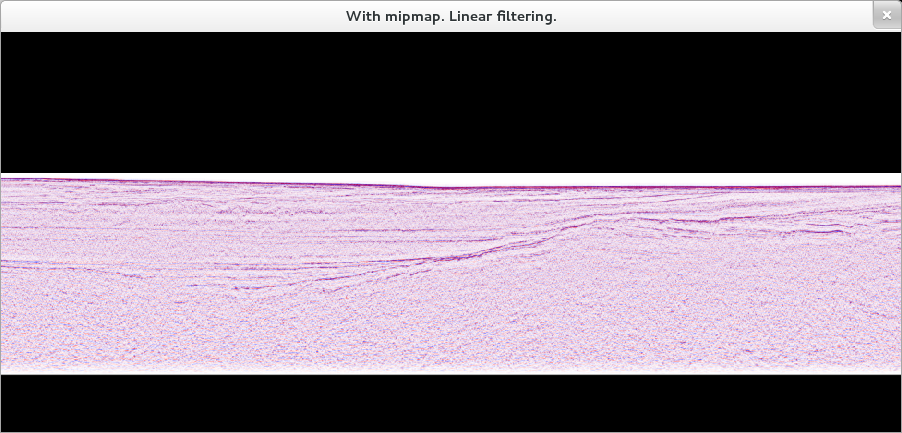
\includegraphics[clip=true, trim=10cm 5cm 10cm 6.5cm]{graphics/mip-on_linear_z0.7_x0.0_y0.0.png}
\caption{Mipmapping; linear filtering.}
\label{fig:mip_lin}
\end{figure}


\begin{figure}[htp]
\centering
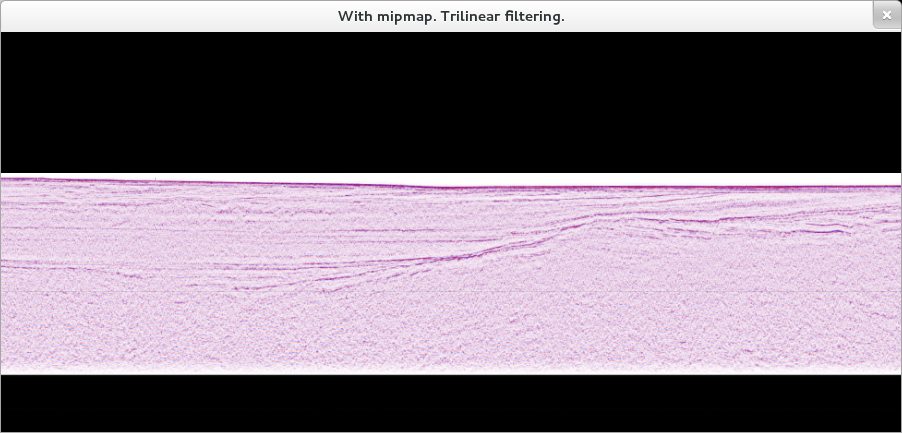
\includegraphics[clip=true, trim=10cm 5cm 10cm 6.5cm]{graphics/mip-on_trilinear_z0.7_x0.0_y0.0.png}
\caption{Mipmapping; trilinear filtering.}
\label{fig:mip_trilin}
\end{figure}


\begin{figure}[htp]
\centering
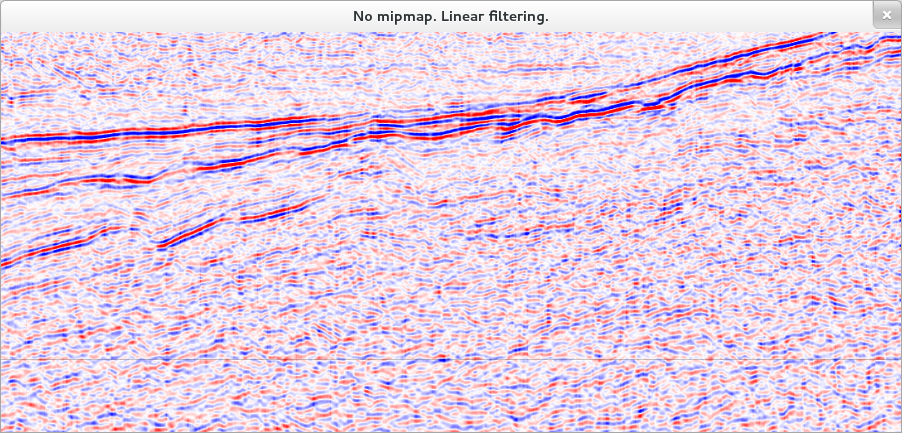
\includegraphics[clip=true, trim=10cm 5cm 10cm 6.5cm]{graphics/mip-off_linear_z0.1_x0.0_y0.7.png}
\caption{No mipmapping; linear filtering. Zoomed in.}
\label{fig:no_mip_lin_zoomed-in}
\end{figure}


\begin{figure}[htp]
\centering
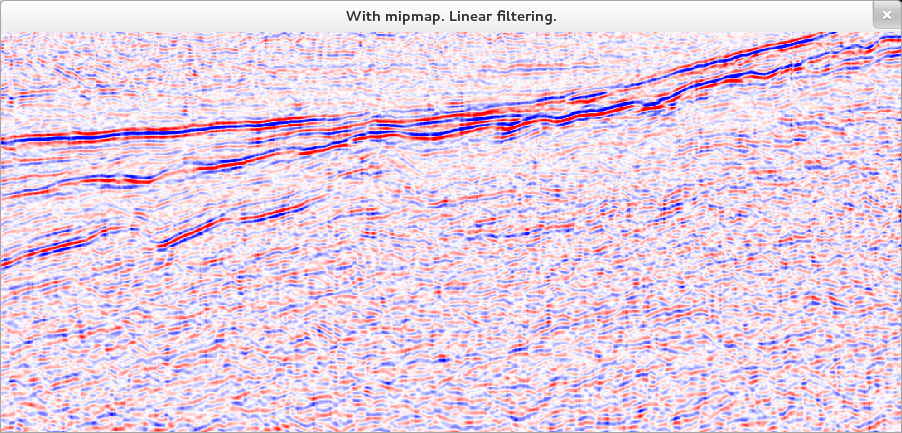
\includegraphics[clip=true, trim=10cm 5cm 10cm 6.5cm]{graphics/mip-on_linear_z0.1_x0.0_y0.7.png}
\caption{Mipmapping; linear filtering. Zommed in.}
\label{fig:mip_lin_zoomed-in}
\end{figure}


% section mipmap_and_filter (end)


\end{document}















































